\section{L'équipe de Data Publica}
    \subsection{L'équipe technique}
    \label{annexe:teamd_data_publica}
        L'équipe technique de Data Publica est visible en figure \ref{fig:teamd_data_publica}.
        \begin{figure}[h!]
            \centering
            \begin{subfigure}[b]{0.2\textwidth}
                
\includegraphics[width=\textwidth]{images/christian-serieux.png}
                \caption{Christian F.}
                \label{fig:christian}
            \end{subfigure}
            \begin{subfigure}[b]{0.2\textwidth}
                
\includegraphics[width=\textwidth]{images/thomas2-Copier-Copier.jpg}
                \caption{Thomas D.}
            \end{subfigure}
            \begin{subfigure}[b]{0.2\textwidth}
                
\includegraphics[width=\textwidth]{images/guillaume-serieux.png}
                \caption{Guillaume L.}
            \end{subfigure}
            \begin{subfigure}[b]{0.2\textwidth}
                
\includegraphics[width=\textwidth]{images/samuel-serieux.png}
                \caption{Samuel C.}
            \end{subfigure}
            \begin{subfigure}[b]{0.2\textwidth}
                
\includegraphics[width=\textwidth]{images/loic-serieux.png}
                \caption{Loïc P.}
            \end{subfigure}
            \begin{subfigure}[b]{0.2\textwidth}
                
\includegraphics[width=\textwidth]{images/clement-c-serieux.png}
                \caption{Clément C.}
            \end{subfigure}
            \begin{subfigure}[b]{0.2\textwidth}
                
\includegraphics[width=\textwidth]{images/clement-d-serieux.png}
                \caption{Clément D.}
            \end{subfigure}
            %\begin{subfigure}[b]{0.2\textwidth}
            %    
\includegraphics[width=\textwidth]{images/jacques.jpg}
            %            \caption{Jacques B.}
            %\end{subfigure}
            \begin{subfigure}[b]{0.2\textwidth}
                
\includegraphics[width=\textwidth]{images/vincent.jpg}
                \caption{Vincent Y.}
            \end{subfigure}
            \caption{L'équipe technique de Data Publica}
            \label{fig:teamd_data_publica}
        \end{figure}

\newpage

    \subsection{L'équipe commerciale}
    \label{annexe:teamc_data_publica}
        L'équipe commerciale de Data Publica est visible en figure \ref{fig:teamc_data_publica}.
        \begin{figure}[h!]
            \centering
            \begin{subfigure}[b]{0.2\textwidth}
                
\includegraphics[width=\textwidth]{images/francois-serieux.png}
                \caption{François B.}
                \label{fig:francois}
            \end{subfigure}
            \begin{subfigure}[b]{0.2\textwidth}
                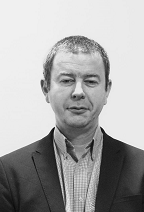
\includegraphics[width=\textwidth]{images/emmanuel-serieux.png}
                \caption{Emmanuel J.}
            \end{subfigure}
            \begin{subfigure}[b]{0.2\textwidth}
                
\includegraphics[width=\textwidth]{images/philippe-1-serieux.png}
                \caption{Philippe S.}
            \end{subfigure}
            \begin{subfigure}[b]{0.2\textwidth}
                
\includegraphics[width=\textwidth]{images/Justine-serieuse-crop.jpg}
                \caption{Justine P.}
            \end{subfigure}
            \caption{L'équipe commerciale de Data Publica}
            \label{fig:teamc_data_publica}
        \end{figure}

\section{Dataviz}
\label{annexe:firmo}
    Un exemple de dataviz est présenté en figure \ref{fig:firmo}.
    \begin{figure}[h!]
        \centering
        
\includegraphics[width=\textwidth]{images/firmo.jpg}
        \caption{Exemple de Dataviz : Firmographie dans C-Radar}
        \label{fig:firmo}
    \end{figure}

\section{La validation croisée et les hyper-paramètres}
    \subsection{Les hyper-paramètres}
    \label{annexe:hyper_param}

    \subsection{La validation croisée}
    \label{annexe:cv}
        La validation croisée est une technique de validation indiquant comment les résultats d'une analyse statistique se généralisent à un ensemble de données indépendant. Cette dernière est particulièrement utilisée lorsque l'on souhaite estimer la précision d'un modèle prédictif en pratique. En générale, dans les problèmes de prédiction, un modèle est construit avec un ensemble de données d'apprentissage, et ensuite un autre ensemble de données (jamais vu du modèle) sont utilisées pour tester le modèle. Le but de la validation croisée est de définir un ensemble de données utilisé pour tester le modèle durant sa phase d’entraînement (de construction). L'ensemble de données de validation est utilisé pour éviter les problèmes de sur-apprentissage et pour donner un aperçu de comment le modèle va se généraliser à un ensemble de données indépendant (un ensemble de données inconnu).\\

        Un plis de validation croisée consiste à partitionner un échantillon des données en deux sous-ensembles. Le premier permet d'effectuer l'analyse sur celui-ci (appelé l'ensemble d'apprentissage), et le second de valider l'analyse sur celui-là (appelé l'ensemble de validation ou de test). Pour réduire l'incertitude, de multiples plis de validation croisée sont effectué en partitionnant l'ensemble de données en plusieurs partitions utilisées à chaque plis. Les résultats de la validation sont moyennés sur les différents plis.\\

        La validation croisée est importante pour évaluer la qualité et la capacité de généralisation d'un modèle surtout lorsque les données sont rares ou difficiles à collecter.\\

        L'une des raisons principales pour laquelle on l'utilise, plutôt qu'une méthode plus traditionnelle (consistant à partitionner l'ensemble de données en deux ensembles, 70\% de l'ensemble pour la phase d'apprentissage et 30\% pour la phase de test), est la suivante : Dans une validation traditionnelle, l'erreur sur l'ensemble d'apprentissage n'est généralement pas un bon estimateur de la performance du modèle, de même que l'erreur sur l'ensemble de test. Celles-ci ne décrivent pas totalement la performance du modèle. C'est le cas lorsqu'il n'y a pas suffisamment de données disponibles ou lorsque la distribution et la disparité des données à partitionner ne sont pas bonnes en phase d'apprentissage et de test.\\

        Les deux techniques de validation croisée s'appellent :
        \begin{itemize}
            \item \textit{Leave-p-out cross-validation} : méthode la plus traditionnelle ;
            \item \textit{k-fold cross-validation} : autre méthode décris ci-dessus fonctionnant par plis.
        \end{itemize}

    \subsection{La validation croisée stratifiée}
    \label{annexe:cv_s}
        Lors du partitionnement de l'ensemble de données en k sous-ensembles, la validation croisée stratifiée  garantit que la proportion des classes soit conservée dans les k sous-ensembles résultant. De plus, l’ensemble est mélangé à chaque nouvelle construction du modèle avant d'être diviser en k sous-ensembles.

\section{Les métriques de mesure de la qualité d'une classification}
    \subsection{Terminologies}
        Pour une classe donnée, voici la signification de ces terminologies :
        \begin{itemize}
            \item $\highlight[green]{TP}$ : True positive, bonne assignation à la classe ;
            \item $\highlight[green]{TN}$ : True negative, bon rejet de la classe ;
            \item $\highlight[red]{FP}$ : False positive, mauvaise assignation à la classe ;
            \item $\highlight[red]{FN}$ : False negative, mauvais rejet de la classe.
        \end{itemize}

    \subsection{La précision}
    \label{annexe:precision}
        Pour une classe donnée, la précision est le nombre de documents correctement assignés à cette classe rapporté au nombre de documents total assignés à cette classe par le classifieur.\\
        $Précision\ =\ \frac{TP}{TP+FP}$


    \subsection{Le rappel}
    \label{annexe:rappel}
        Pour une classe donnée, le rappel est défini par le nombre de documents correctement assignés à cette classe au regard du nombre total de documents appartenant réellement à cette classe.\\
        Le rappel mesure le fait que le classifieur ait trouvé tous les documents d'une classe.\\
        $Rappel\ =\ \frac{TP}{TP+FN}$

\section{Les stratégies de modèles de classification en contexte multi-classe}
    \subsection{One versus All}
    \label{annexe:one_vs_all}

    \subsection{One versus One}
    \label{annexe:one_vs_one}


\section{Le QA ou Quality Assessment}
\label{annexe:qa}
    L'objectif du QA est de demander la contribution d'un maximum de personnes sur une tâche de validation manuelle pénible.\\

\section{Modèle de classifieur}
    Les points d'explication qui suivent, sont en partie tirés de Wikipédia\autocite{wiki_discri_gene}.
    \subsection{Le modèle génératif}
    \label{annexe:generatif}
        Le modèle génératif consiste à modéliser les probabilités conditionnelles soit $P(donnée | classe)$. Voici quelques exemples d'algorithmes de ce type :
        \begin{itemize}
            \item Classifieur naïf bayésien implique une distribution de probabilité conditionnelle de type binomiale (ou multinomiale) ;
            \item Analyse discriminante linéaire (LDA). Elle implique l'existence d'un modèle discriminant basé sur une distribution de probabilité de type Gaussienne.
        \end{itemize}
        Le modèle génératif maximise la vraisemblance de la probabilité jointe $P(classe, donnée)$.

    \subsection{Le modèle discriminant}
    \label{annexe:discriminatif}
        Le modèle discriminant cherche à maximiser la qualité de la classification. Une fonction de coût va réaliser l'adaptation du modèle de classification (en minimisant les erreurs). Voici quelques exemples d'algorithmes de ce type :
        \begin{itemize}
            \item Régression logistique, maximisation de la vraisemblance en considérant que les données suivent un modèle binomial ;
            \item Support Vectort Machine (SVM), maximisation de la marge entre l'hyperplan séparant les données.
        \end{itemize}
        Le modèle discriminant maximise la vraisemblance de la probabilité conditionnelle $P(classe | donnée)$.

\section{Les transducteurs}
\label{annexe:transducteurs}
    Définition tirée de Wikipédia\autocite{wiki_trans}.\\

    En informatique théorique, en linguistique, et en particulier en théorie des automates, un transducteur fini (appelé aussi transducteur à états finis par une traduction maladroite de l'anglais finite state transducer) est un automate fini avec sorties. C'est une extension des automates finis. Ils opèrent en effet sur les mots sur un alphabet d'entrée et, au lieu de simplement accepter ou refuser le mot, ils le transforment, de manière parfois non déterministe, en un ou plusieurs mots sur un alphabet de sortie. Ceci permet des transformations de langages, et aussi des utilisations variées telles que notamment l'analyse syntaxique des langages de programmation, et l'analyse morphologique ou l'analyse phonologique en linguistique.\\

    D'autres explications détaillées sont disponibles \href{http://sixty-north.com/blog/deriving-transducers-from-first-pr}{ici}.